
%\documentclass[10pt,journal,compsoc]{IEEEtran}
\documentclass[format=sigconf, review=false, anonymous=false]{acmart}
%\documentclass[acmlarge]{acmart}
%\usepackage{cite}
%\usepackage[pdftex]{graphicx}
%\usepackage[table]{xcolor}
\usepackage{booktabs}
%\usepackage{float}
%\usepackage{subfig}
\usepackage{subcaption}
\usepackage{graphicx}
\usepackage{tabularx}	
\usepackage{balance}
\usepackage{makecell}
\usepackage{array}
\usepackage{tablefootnote}
\usepackage{footnote}
\usepackage{graphicx}
\usepackage{textcomp}
\usepackage{float}

\usepackage{tikz}
\usepackage{xcolor}
\newcommand*\circled[1]{\tikz[baseline=(char.base)]{
            \node[shape=circle,draw,inner sep=2pt] (char) {#1};}}

\fancyfoot{}


\setcopyright{acmcopyright}
%\copyrightyear{2019}
%\acmYear{2019}
%\acmConference[MEMSYS '19]{Proceedings of the International Symposium on Memory Systems}{September 30-October 3, 2019}{Washington, DC, USA}
%\acmBooktitle{Proceedings of the International Symposium on Memory Systems (MEMSYS '19), September 30-October 3, 2019, Washington, DC, USA}
%\acmPrice{15.00}
%\acmDOI{10.1145/3357526.3357531}
%\acmISBN{978-1-4503-7206-0/19/09}

\settopmatter{printacmref=false} % Removes citation information below abstract
\renewcommand\footnotetextcopyrightpermission[1]{} % removes footnote with conference information in first column
\pagestyle{plain} % removes running headers

\def\fixme#1{\bgroup \color{red}{[{#1}]}\egroup}
\def\pr#1{\bgroup \color{blue}{[PR,{#1}]}\egroup}

\def\ka#1{\bgroup \color{purple}{[KA,{#1}]}\egroup}

\begin{document}

\title{Evaluating HPC Kernels for Processing in Memory}

\author{Kazi Asifuzzaman, Mohammad Alaul Haque Monil, Frank Liu, Jeffrey S Vetter}
\affiliation{
  \institution{Oak Ridge National Laboratory, USA}}

% \author{Kazi Asifuzzaman}
% \affiliation{%
%   \institution{Oak Ridge National Laboratory, USA}}

% \author{Mohammad Alaul Haque Monil}
% \affiliation{%
%   \institution{Oak Ridge National Laboratory, USA}}

% \author{Frank Liu}
% \affiliation{%
%   \institution{Oak Ridge National Laboratory, USA}}

% \author{Jeffrey S Vetter}
% \affiliation{%
%   \institution{Oak Ridge National Laboratory, USA}}



\renewcommand{\shortauthors}{}

\begin{CCSXML}

<ccs2012>
<concept>
<concept_id>10010520.10010575.10010580</concept_id>
<concept_desc>Computer systems organization~Processors and memory architectures</concept_desc>
<concept_significance>300</concept_significance>
</concept>
\end{CCSXML}

\ccsdesc[300]{Computer systems organization~Processors and memory architectures}

%\printccsdesc

\begin{abstract}
	Abstract goes here... 
\end{abstract}

\keywords{Processing in Memory, High Performance Computing}






\maketitle
\thispagestyle{empty}

\section{Introduction}
Memory systems are dominant factors in large scale High Performance Computing (HPC) clusters in terms of performance and energy consumption. It also significantly contributes to the setup and operational cost of such systems. Dynamic Random Access Memory or DRAM technology has been adopted and served as the primary building blocks of main memory sub systems on the majority of computing domains including HPC. DRAM in its conventional organization (i.e. DIMMs) is struggling accommodate the exceeding memory requirements of emerging applications from different domains. This is primarily due to the fact that main memory systems and computing units are clearly separate devices and they are usually located far apart and communicate via buses that are constrained by a limited number of pins. In addition, DRAM devices usually operates in much lower frequency than the compute units (CPU/GPU). As a results, accessing the main memory for reading and writing memory blocks are expensive operations in terms of latency and energy consumption. To give a perspective, accessing data data from a DRAM device to the processing unit through the cache hierarchy takes about two orders of magnitude more energy than performing a floating point point operation in a processor. Over the years, several techniques have been adopted to complement the penalty occurring from memory operations. Several layers of cache hierarchy is introduced to reduce accesses to the main memory. Out-of-order cores are expected to continue execution while its waiting for the data from the main memory. Despite the efforts, memory access overhead continues to sustain as a major bottleneck for efficient execution of applications in HPC and other domains.

Researchers are investigating alternative solutions to keep up with the increasing memory demands from modern applications. Part of that effort focuses on using novel memory technologies based on new materials such as Phase Change Memory (PCM), Spin-Transfer-Torque Magnetic RAM (STT-MRAM), Resistive RAM (ReRAM) etc. The idea is to leverage unique properties of these memory technologies (non-volatility, endurance, no leakage current) to come up with an efficient alternative to DRAM technology. However, significant development at the cell/material level is warranted to get these memory technologies ready to attain DRAM-like performance. In addition, such extensive research and development efforts would also induce cost overhead for these technologies and it would be increasingly difficult to be commercially viable against very affordable DRAM technology.   
%be deployed and
The other approach is to change the organization of conventional memory systems using the same DRAM technology. 3D stacking of DRAM dies appears to be a convenient way to increase capacity and moving the stack closer to the CPU on the same silicon interposer greatly helps to reduce the memory access latency. Silicon interposer also allows to have denser buses (e.g. 1024 bits) between memory stack and processing unit, effectively increasing the bandwidth. Currently, High bandwidth Memory (HBM) and Hybrid Memory Cube (HMC) are the two major protocols adopting that adopt 3D stacking DRAM model.        

HMC comes with an optional logic layer beneath the stack. This logic layer can be leveraged to implement simple processing units closer to the memory, which corresponds to the technique Processing-in-memory (PIM)\footnote{Also known as Compute-in-Memory (CIM), processing-near-memory or processing-using-memory. For simplicity we refer to it as Processing-in-memory (PIM) throughout the paper.}, which builds on the idea of moving the execution of certain memory-intensive applications/kernels to the memory, instead of bringing the data to CPU for processing through expensive memory accesses. An upsurge of research activity investigating different PIM techniques indicates that it has significant potential to accelerate memory bound problems. Recent studies report significant improvements in performance and energy efficiency by adopting PIM techniques. However, these studies largely focus and analyze on the applications from Artificial Intelligence, Machine Learning, Neural Network domain along with some generic kernels. 

In this paper, we perform a preliminary evaluation of HPC kernels for Processing in Memory. We select five HPC benchmarks applications developed by laboratories of US Department of Energy (DoE) along with two well-known generic applications, identify their memory intensive kernels and analyze their suitability and performance with processing-in-memory. We further extend our experiments to examine several other special kernels and investigate how their performance on PIM compare with the memory-intensive kernels.   

The rest of the paper is organized as follows. Section 2 presents a brief background on PIM techniques, Section 3 presents the workload characterization of target applications, Section 4 explains the experimental setup and methodologies used, Section 5 presents the results of the evaluation, Section 6 discusses related studies and Section 7 summarizes the conclusions of the study.   
  

\section{Background}
Processing in memory generally refers to the idea of moving some of the executions to the memory unit, when moving the data to the CPU for processing deem to take more time, which is often the case for memory intensive kernels. With various memory technologies and PIM optimization techniques present, there are several ways PIM can be adopted. Figure~\ref{fig:pimcat} shows a generic representation of a main memory DIMM module. A main memory DIMM (e.g. DDR4 DIMM) has several chips. Each each has a number of banks (e.g. 4, 8, 16) and each bank has a specified number of rows and columns which constitutes the memory array (highlighted as \circled{1} in Figure ~\ref{fig:pimcat}). Each intersection of a row and column typically represents a memory \textit{cell} which holds single bit data. When a row address is requested to be accessed, that selected row is then loaded on to the row buffer (highlighted as \circled{2}) %in Figure ~\ref{fig:pimcat}).







-	PIM background \\
-	Different types of PIM \\
-	Which type of PIM can be beneficial for HPC \\


\begin{figure}[t!]
\centering
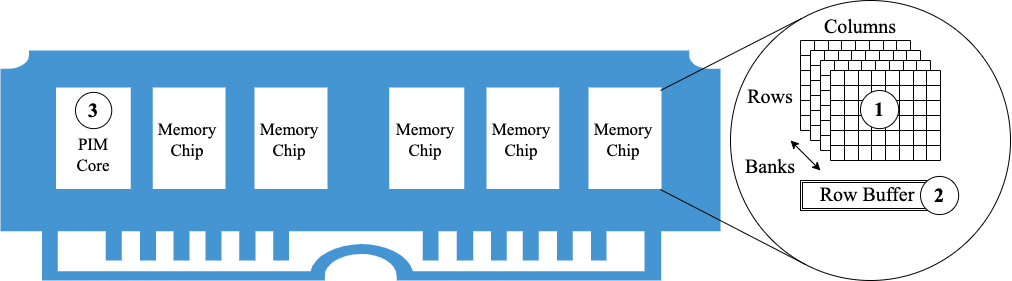
\includegraphics[width=\columnwidth]{MEMSYS22/figures/pimcat.png}
%\vspace{.5em} 
\caption{Generic representation of a Main Memory DIMM and where processing in memory can take place.}
%\vspace{-1.5em} 
\label{fig:pimcat}
%\vspace{-0.6cm}    
\end{figure}   
\looseness -1


    

\section{Workload Characterization of HPC applications}
\label{sec:workload}

-	Roofline model \\
-	Identifying functions that are memory intensive \\

\subsection{Jacobi}
The main function in Jacobi is the $stencil\_jacobi$ function which is a memory bound kernel (see Fig.~\ref{fig:roof-jacobi}). 

\begin{figure}[h]%[bp]
\begin{center}
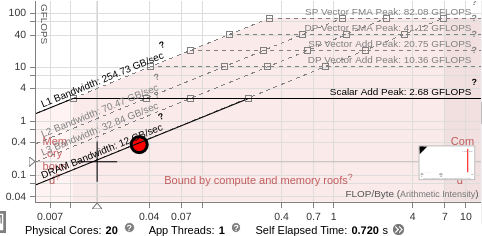
\includegraphics[width=1\linewidth]{MEMSYS22/figures/roofline/jacobi.png}
\end{center}
  \vspace{-0.1in}
\caption{Positioning of Jacobi kernel in Roofline}
\label{fig:roof-jacobi}
\vspace{-0.2in}
\end{figure}

%\begin{figure}[t!]
%\centering
%\includegraphics[width=70mm, height= 50mm]{figure/pmtj.pdf}
%%\vspace{.5em} 
%\caption{STT-MRAM cell}
%%\vspace{-1.5em} 
%\label{fig:pmtj}
%%\vspace{-0.3cm}   
%\end{figure} 
%
%
%
%
%  
%\looseness -1
%
%
%
%\begin{figure}[t!]
%\centering
%\includegraphics[width=\columnwidth]{figure/DeviceCapacity.pdf}
%%\vspace{.5em} 
%\caption{DRAM and STT-MRAM capacity growth in years} %\pr{23-Feb: Kazi, do we have any data from after 2016? Take care of this only if you have some extra time. }}
%%\vspace{-1.5em} 
%\label{fig:Capa}
%\vspace{-0.3cm}  
%\end{figure}  


%
%
%\begin{table}[t!]
%%\normalsize
%\small
%\caption{\mbox{DRAM vs STT-MRAM for embedded real-time systems}}
%\centering
%%    \begin{tabularx}{\columnwidth}{lcc}
%    \begin{tabularx}{7.2cm}{lcc}
%\toprule
%    % \hline
%    Feature & DRAM & STT-MRAM \\
%\midrule
%Radiation-hard & - & +++ \\
%Standby power  & - & +++ \\
%Temperature tolerance & + & +++ \\
%Storage capacity & ++ & ++ \\
%Access speed   & +++ & ++ \\
%Endurance      & ++ & +++ \\
%\bottomrule
%   \end{tabularx}
%\label{table:compare}
%%\vspace{-0.5cm}
%\end{table}
%
%
%
%\begin{figure}[t!]
%\centering
%\includegraphics[width=\columnwidth]{figure/processor.png}
%\caption{Schematic view of the Next Generation Microprocessor~(NGMP)}
%\label{fig:processor}
%%\vspace{-0.4cm}
%\end{figure}









  

\section{Experimental environment}
\label{sec:Experimental}



%In this section we describe the simulator infrastructure target hardware platform, , and benchmarks used to carry out the experiments.

For our experiments we use recently released DAMOV-SIM simulation infrastructure~\cite{71}. DAMOV is based on ZSim system simulator[] coupled with Ramulator memory simulator[]. ZSim is used simulate both host and pim core's microarchitecture, cache hirerchy and coherence protocols; whereas Ramulator models HMC main memory architecture, memory controller and main memory access protocols. The system configurations used in the simulations are summarized in Table~\ref{table:hostarch}. DAMOV-SIM uses pintool v. 2.14, on a Linux kernel v.3.8.  

First we identify the memory intensive kernels of the benchmarks under study, as detailed in Section 3. We use DAMOV-SIM's offloading support to isolate identified functions by inserting delimiter functions and run them for 1 billion instructions. In the configuration file, when \texttt{pimMode} is set to \texttt{true} Zsim simulates a pim core with shorter latency to memory with high bandwidth. When \texttt{pimMode} is set to \texttt{false} it simulate a core with regular settings (host processor). At function-level offloading granularity it is easier to determine and comapre how the same function performs in PIM and host cores. %The simulation infrastructure does not yet support concurrent execution on PIM and host core.         

The simulation infrastructure provides three important performance matrices: Instruction Per Cycle (IPC), Misses-Per-Kilo-Instruction (MPKI) and Last to First Miss Ratio (LFMR), which indicates the ratio of last level cache misses to first level cache misses.    




%DAMOV-SIM supports function offloading using Zsim delimiters.     




% \subsection{DAMOV}
% - Host CPU Configuration \\
% - PIM CPU configuration \\
% \subsection{HMC}
% - Configuration \\


% \begin{savenotes}
%\begin{table}[t!]
%%\vspace{-0.5cm}
%%\normalsize
%\small
%\caption{DRAM and STT-MRAM parameters associated with row operation (DDR2-667 cycles)}
%%\begin{center}
%    
%    \begin{tabularx}{\columnwidth}{@{}lXrrrr}
%\toprule
%    % \hline
%    Timing \\Parameters & Description & \tiny{DRAM} & \tiny{ST-1.2} & \tiny{ST-1.5} & \tiny{ST-2.0}\\
%\midrule
% tRCD & \mbox{Row to column} \mbox{command delay} & 5 & 6 & 8 & 10\\
% tRP & Row precharge & 5 & 6 & 8 & 10\\
% tFAW & Four row \mbox{activation window} & 13 & 16 & 20 & 26\\
% tRRD & Row to Row \mbox{activation delay} & 3 & 4 & 5 & 6\\
% tRFC & \mbox{Refresh cycle time} & 43 & 0 & 0 & 0\\
%\bottomrule
%   \end{tabularx}
%
%\label{table:ROW}
%\end{table}
%   \end{savenotes}
%
%
%
%
%% 
%
\begin{table}[t!]
%\normalsize
\small
\caption{Configurations used in the simulation }
%\begin{cente
    \begin{tabularx}{\columnwidth}{lXr}
\toprule
    % \hline
Unit & Configuration  \\
\midrule
Host CPU & 1 out-of-order Core running at 2.4GHz,   \\
L1 Cache & 32KB, 8-way, 64B/Line, LRU policy \\
L2 Cache & 256KB, 8-way, 64B/Line, LRU Policy \\
L3 Cache & 8MB, 16-way, 64B/Line, LRU Policy  \\
\midrule
PIM CPU & 1 out-of-order Core running at 2.4GHz,   \\
L1 Cache & 32KB, 8-way, 64B/Line, LRU policy \\
\midrule
Main Memory & HMC v.2.0, 32 Vaults, 8 DRAM banks/vault, 256B row buffer, 8GB capacity.\\


\bottomrule
  \end{tabularx}
\label{table:hostarch}
%\vspace{-4mm}
\end{table}
%
%
%
%\begin{figure}[t!]
%\centering
%\includegraphics[width=\columnwidth]{figure/pWCET.png}
%\caption{
%%\textbf{X-axis:} pWCET: Probabilistic worst case execution time (pWCET); 
%%\textbf{Y-axis:} Exceedance probability; 
%%\textbf{Caption:} 
%pWCET distribution: Probability (Y-axis) that the application execution
%time (in any given run) exceeds the corresponding time on the X-axis.
%	In this example, the pWCET estimate (7ms) is exceeded with a probability of $10^{-12}$.}
%\label{fig:pWCET}
%%\vspace{-5mm}
%\end{figure}
%
%
%\begin{figure}[t!]
%\centering
%\includegraphics[width=\columnwidth]{figure/MBPTA-CV.png}
%\caption{
%Schematic of the MBPTA application process}
%\label{fig:MBPTA-CV}
%%\vspace{-5mm}
%\end{figure}
%
%
%
%
%
%\subsection{Benchmarks}
%
%\begin{table}[t!]
%%\normalsize
%\small
%\caption{Benchmarks used in the study}
%%\begin{center}
%    \begin{tabularx}{\columnwidth}{lXrrrr}
%\toprule
%    % \hline
%    Suite & Benchmarks & Domain \\
%    
%\midrule
%ESA Applications & obdp, debie & Space\\
%\midrule
%EEMBC Autobench & a2time01, aifftr01, aifirf01, aiifft01, basefp01, bitmnp01, cacheb01, canrdr01, idctrn01, iirflt01, matrix01, pntrch01, puwmod01, rspeed01, tblook01, ttsprk01 & Automotive\\
%\midrule
%Mediabench & mesa.texgen, mesa.mipmap, epic.decode, mesa.osdemo & Media \\
%\bottomrule
%   \end{tabularx}
%\label{table:benchmark}
%\end{table}
%  




\section{Evaluation}
\label{sec:evaluation}
-	Performance gain (IPC) \\
-	LFMR, MPKI \\
-	Energy  \\

%
%\begin{figure}[t!]
%\hspace*{-9.5cm}
%\centering
%\includegraphics[width=\textwidth, height=60mm]{figure/Set1.pdf}
%%\caption{ST-1.2 Configuration (floating point benchmarks): Speedup ranges from 0\% (tonto) to 7.4\% (milc), and it is 2.7\% on average.}
%\label{fig:Set1}
%\end{figure}
%
%
%\begin{figure}[htbp]
%  
%\centering
%\includegraphics[width=\textwidth, height=60mm]{figure/Set2.pdf}
%%\caption{ST-1.2 Configuration (floating point benchmarks): Speedup ranges from 0\% (tonto) to 7.4\% (milc), and it is 2.7\% on average.}
%\label{fig:Set2}
%\end{figure}
%
%
%\begin{figure*}[t!]
%\centering
%\includegraphics[width=\textwidth, height=60mm]{figure/Set3.pdf}
%%\caption{ST-1.2 Configuration (floating point benchmarks): Speedup ranges from 0\% (tonto) to 7.4\% (milc), and it is 2.7\% on average.}
%\label{fig:Set3}
%\end{figure*}
%
%%\vspace{5cm}
%\newpage
%
%\begin{figure}[H]
%\centering
%\includegraphics[width=\textwidth, height=60mm]{figure/Set4.pdf}
%%\caption{ST-1.2 Configuration (floating point benchmarks): Speedup ranges from 0\% (tonto) to 7.4\% (milc), and it is 2.7\% on average.}
%\label{fig:Set4}
%\end{figure}










%\section{Related work}
%\label{sec:RelatedWork}
%Several recent studies explore the architectural scope and application domains of processing in memory.

\subsection{Architectural Scope of PIM}

Processing in the memory array is addressed in several studies~\cite{03,06,13,15,20,29}. Leitersdorf et al. \cite{13} propose to improve in-memory multiplication with partition-based computation techniques for broadcasting and moving data within partitions. The authors exploit ReRAM's voltage controlled variable resistance to support logic gates. Long et al. \cite{20} proposes another ReRAM based design particularly for Recurrent Neural Network (RNN) acceleration. The study proposes crossbar sub-arrays for vmatrix vector multiplication, multiplier sub-arrays for element-wise operations and special function units for nonlinear functions. Peng et al. \cite{15} present a new mapping method and data flow to maximize reuse of weight and input data on a 8-bit ReRAM based PIM architecture. 
Lin et al. \cite{31} present PIM design proposing optimization at the row buffer level. The authors introduce a \textit{Population Count Engine} which works on the data inside the sense amplifier and store the results back to the sense amplifier. Majority of the studies adopt near memory compute unit equipped with simple core(s) \cite{01,02,05,11,12,17,30,32,33,34,35}. Lee et al. \cite{12} develops an industrial prototype of a PIM design that can seamlessly work with a variety of commercial processors without requiring any changes on the applications. The proposed PIM execution unit has a five-stage pipeline, 16-wide SIMD FPU, registers and controller. This design is based on a HBM stack which is fabricated with a 20nm technology process. PimCaffe \cite{16} develops a PIM near memory design based on multiple FPGAs, implementing SIMD and systolic array compute engines for vector and matrix multiplications.       

\subsection{Application Domain}

The vast majority of the studies attempts to accelerate application segments from Machine Learning, AI and Neural Network domain \cite{03,04,08,09,10,11,14,15,16,18,19,20,22,29,31}. Since applications from these domains frequently use matrix vector multiplication operations, where the coefficients can be naturally mapped to the word-lines (WL) and bit-lines (BL) and use the data array to compute the dot product in the each cell then eventually accumulating them along the source-lines (SL) \cite{15,20}. In another approach few studies use the logic die of 3D stacked memories to place Processing Elements (PE) directly beneath the DRAM dies with shorter distance to the coefficient data for faster computation in each layer [09,22]. Imani et al. \cite{6} report to have achieved graph processing and query processing capabilities along with machine learning acceleration with processing in memory. Huang et al. \cite{33} propose a heterogeneous PIM design incorporating memristors and CMOS based technologies, in order to accommodate the heterogeneity requirements of graph applications. DAMOV~\cite{71} is a PIM simulation infrastructure based ZSim[] and Ramulator[] with offloading support. The authors develops a rigorous workload characterization methodology and quantify data movement bottleneck on an extensive set of applications and functions.     

 

\section{Conclusions}
\label{sec:Conclusions}
In this paper, we perform a first-order evaluation of HPC kernels developed by laboratories of US Department of Energy (DoE) for processing-in-memory (PIM) technique. To that end, we characterize seven HPC applications and identify memory-intensive kernels which we run on host core and PIM core with HMC main memory module using DAMOV-SIM simulation infrastructure. The results show that two out of the seven HPC kernels achieve a performance gain executing in the PIM core, which is largely analogous to the L3 misses per kilo instructions (MPKI) of each kernel. The results also suggests that MPKI is not the only factor that determines if a kernel would benefit from executing on a PIM core. We observe that a kernel may perform relatively better on a PIM core than another kernel with a higher MPKI but having a lower LFMR.  

%\section{Acknowledgment}

%This work was supported by ....


%\balance
%\bibliographystyle{ACM-Reference-Format}
\bibliographystyle{unsrt}
%\bibliographystyle{acm}
%\bibliographystyle{agsm}
%\bibliographystyle{abbrv}
%\bibliographystyle{IEEEtranS}
\bibliography{RTST_paper} 


\end{document}



